\documentclass[12pt,a4paper]{article}
\usepackage[utf8]{inputenc}
\usepackage[T1]{fontenc}
\usepackage[brazil]{babel}
\usepackage{geometry}
\geometry{a4paper, top=2.5cm, bottom=2.5cm, left=2.5cm, right=2.5cm}

\usepackage{times}
\usepackage{graphicx}
\usepackage{amsmath, amssymb}
\usepackage{booktabs}
\usepackage{multirow}
\usepackage{float}
\usepackage{subcaption}
\usepackage{caption}
\usepackage{xurl}
\usepackage{hyperref}

\graphicspath{{./figures/}}

% Configuração dos hyperlinks
\hypersetup{
    colorlinks=true,
    linkcolor=blue,
    citecolor=blue,
    urlcolor=blue,
    pdftitle={Relatório TP2 - Algoritmos 2},
    pdfauthor={Cauã Neto Santos Pires, Rafael Junqueira Baracat, Renato Vilela de Melo},
    pdfsubject={TP2 - Análise Empírica e Otimização para o Caixeiro Viajante}
}

\begin{document}

% =========================
% CAPA
% =========================
\begin{titlepage}
    \centering
    {\Large DCC207 - Algoritmos 2}\\[1.5cm]
    {\Huge \textbf{Trabalho Prático 2}}\\[0.5cm]
    {\LARGE Análise Empírica e Otimização para o Caixeiro Viajante}\\[2cm]

    \vfill
    \textbf{Alunos:} \underline{Cauã Neto Santos Pires, Rafael Junqueira Baracat, Renato Vilela de Melo} \\[0.5cm]
    \textbf{Matrículas:} \underline{2024005335, 2024066024, 2024066016} \\[3cm]

    {\large ICEx -- UFMG \\ 2026/2}
\end{titlepage}

% =========================
% SUMÁRIO
% =========================
\tableofcontents
\newpage

% =========================
% 1. INTRODUÇÃO
% =========================
\section{Introdução}

Este trabalho tem como objetivo abordar os aspectos práticos na codificação, a nível de implementação e auditoria, sob a ótica da avaliação de métricas, de algoritmos para problemas computacionalmente difíceis (NP-Difíceis). Para tal, concentramos nossos esforços na aplicação ao Problema do Caixeiro Viajante (TSP) Geométrico (\texttt{EUC\_2D}), investigando três abordagens clássicas:
\begin{itemize}
  \item \textbf{Branch-and-Bound} de saída exata;
  \item \textbf{Twice-around-the-tree} de saída aproximada ($2$-aproximação);
  \item \textbf{Christofides} de saída aproximada ($1{,}5$-aproximação).
\end{itemize}

Não somente isso, auditamos criticamente o uso de estruturas de dados, gargalos teóricos \textit{versus} práticos, o impacto de cinco estratégias de \textit{warm-start} (\textit{Cold Start}, Vizinho Mais Próximo, Inserção por Fecho Convexo, \textit{Twice-around-the-tree} e \textit{Christofides}) na poda da árvore de busca e como a topologia das instâncias impacta o \textit{gap} de aproximação e o colapso da busca exata.

% TODO (Integrante 3): Expandir contextualização sobre o compromisso otimalidade vs. escalabilidade e resumir a organização das seções 2 a 5.

% ==============================================================================
% 2. IMPLEMENTAÇÃO, PROFILING E AUDITORIA
% ==============================================================================
\section{Implementação, Profiling e Auditoria}

\subsection{Arquitetura e Contratos de Dados}
% TODO (Integrante 2): Descrever implementação em Python 3, contratos em src/types.py (TourResult, BnBResult), cálculo de distâncias EUC_2D (floor(d + 0.5)) e isolamento de tracemalloc (track_memory=False por padrão para evitar distorção temporal).

\subsection{Branch-and-Bound: Busca, Limite Inferior e Otimizações}
% TODO (Integrante 2): Detalhar:
% - Escolha de DFS com ordenação de vizinhos vs. Best-First Search (memória O(N) vs. risco de explosão de RAM);
% - Estado leve via bitmask inteiro (zero cópias da matriz de distâncias) e conversão única para dist_list;
% - Quebra de simetria de ciclo em O(1) (exigindo v_1 < v_{N-1});
% - Comparação entre Lower Bounds: two_min O(1) incremental vs. mst O(k^2) com buffers pré-alocados (sem alocação de listas por nó);
% - Controle de timeout (1800s) preservando nós expandidos/podados.

\subsection{Heurísticas de Warm-Start e Algoritmos Aproximados}
% TODO (Integrante 1): Descrever:
% - Cold Start (0 -> 1 -> ... -> N-1 -> 0) e Nearest Neighbor;
% - Convex Hull Insertion (Andrew's Monotone Chain O(N log N) + Cheapest Insertion);
% - Twice-around-the-tree (Prim denso O(N^2) + pré-ordem iterativa com pilha explícita);
% - Christofides (MST + vértices ímpares + Blossom min_weight_matching + circuito euleriano + shortcutting).

\subsection{Auditoria de Código, Refatorações e Gargalos de Sub-rotina}
% TODO (Integrante 1): Relatar as auditorias e refatorações realizadas:
% - Refatoração de convex_hull_insertion de O(N^3) para O(N^2) mantendo cache da melhor aresta;
% - Isolamento de sub-rotinas no Christofides: min_weight_matching cresce de ~38% (N=12) para >90% do tempo total em N=70;
% - Alocação de memória O(N) vs. O(N^2) (subgrafo completo no Blossom e listagens de adjacência).

% ==============================================================================
% 3. METODOLOGIA EXPERIMENTAL
% ==============================================================================
\section{Metodologia Experimental}

\subsection{Ambiente Computacional e Conjunto de Teste (TSPLIB)}
% TODO (Integrante 3): Descrever hardware (Intel Core i5-12500H, Linux, Python 3.12, workers=4), timeout de 1800s (NA) e mediana de 15 repetições com warm-up para heurísticas/aproximados.
% Explicar a composição das 15 instâncias EUC_2D: 12 na Faixa Principal (N <= 40, 80%, subconjuntos topologicamente diversos com ótimos exatos via MILP/DFJ) e 3 na Faixa Limite (eil51, berlin52, st70, 20%).

\subsection{Extração de Features Geométricas e Topológicas}
% TODO (Integrante 3): Definir formalmente as métricas em src/features.py:
% - aspect_ratio do bounding box;
% - convex_hull_ratio (proporção de pontos no fecho convexo);
% - spatial_entropy (entropia de Shannon normalizada em grade fixa 4x4);
% - mst_max_degree e mst_leaf_ratio (estatísticas da MST);
% - nn_dist_cv (coeficiente de variação das distâncias ao vizinho mais próximo).

% ==============================================================================
% 4. EXPERIMENTOS E RESULTADOS
% ==============================================================================
\section{Experimentos e Resultados}

\subsection{Visão Geral de Desempenho e Ponto de Colapso}
% TODO (Integrante 2): Analisar a Tabela 1: 9 de 12 instâncias da Faixa Principal fecharam o ótimo antes de 1800s, enquanto as 3 maiores da Faixa Principal (berlin52_n20, berlin52_n36, st70_n40) e toda a Faixa Limite (N >= 51) atingiram timeout (NA).

\begin{table}[H]
\centering
\caption{Resumo comparativo de tempo de execução (s), nós expandidos e \textit{gap} (\%) nas 15 instâncias \texttt{EUC\_2D} (limite de 1800s no Branch-and-Bound com LB=\texttt{mst}).}
\label{tab:resultados_gerais}
\resizebox{\textwidth}{!}{%
\begin{tabular}{@{}lcccccccc@{}}
\toprule
\multirow{2}{*}{\textbf{Instância}} & \multirow{2}{*}{\textbf{$N$}} & \multirow{2}{*}{\textbf{Ótimo}} & \multicolumn{2}{c}{\textbf{B\&B (Melhor WS)}} & \multicolumn{2}{c}{\textbf{Twice-around-the-tree}} & \multicolumn{2}{c}{\textbf{Christofides}} \\ \cmidrule(lr){4-5} \cmidrule(lr){6-7} \cmidrule(lr){8-9}
 &  &  & \textbf{Tempo (s)} & \textbf{Nós Exp.} & \textbf{Tempo (s)} & \textbf{Gap (\%)} & \textbf{Tempo (s)} & \textbf{Gap (\%)} \\ \midrule
\texttt{eil51\_n12}    & 12 & 123  & 0.0116   & 1.142      & 0.00009 & 16.26 & 0.00039 & 8.13  \\
\texttt{berlin52\_n14} & 14 & 3716 & 0.0435   & 1.251      & 0.00006 & 19.32 & 0.00106 & 3.98  \\
\texttt{st70\_n16}     & 16 & 358  & 0.0015   & 27         & 0.00010 & 13.13 & 0.00059 & 0.00  \\
\texttt{eil51\_n18}    & 18 & 138  & 0.0096   & 374        & 0.00008 & 28.99 & 0.00089 & 7.25  \\
\texttt{berlin52\_n20} & 20 & 3335 & NA       & 64.536.576 & 0.00013 & 7.11  & 0.00112 & 3.84  \\
\texttt{st70\_n22}     & 22 & 318  & 7.0075   & 62.970     & 0.00014 & 15.72 & 0.00295 & 9.75  \\
\texttt{eil51\_n24}    & 24 & 244  & 0.0064   & 114        & 0.00015 & 3.28  & 0.00139 & 4.92  \\
\texttt{berlin52\_n26} & 26 & 2660 & 617.7832 & 3.322.487  & 0.00011 & 36.43 & 0.00155 & 11.84 \\
\texttt{st70\_n28}     & 28 & 305  & 17.1470  & 105.720    & 0.00017 & 30.16 & 0.00227 & 17.38 \\
\texttt{eil51\_n32}    & 32 & 308  & 34.5762  & 386.460    & 0.00013 & 45.45 & 0.00126 & 9.42  \\
\texttt{berlin52\_n36} & 36 & 5760 & NA       & 5.429.248  & 0.00014 & 29.20 & 0.00483 & 14.38 \\
\texttt{st70\_n40}     & 40 & 409  & NA       & 3.042.304  & 0.00016 & 22.98 & 0.00667 & 7.58  \\
\texttt{eil51}         & 51 & 426  & NA       & 10.886.144 & 0.00020 & 42.02 & 0.00520 & 16.67 \\
\texttt{berlin52}      & 52 & 7542 & NA       & 5.429.248  & 0.00020 & 37.92 & 0.00706 & 13.50 \\
\texttt{st70}          & 70 & 675  & NA       & 907.264    & 0.00033 & 29.48 & 0.01332 & 13.33 \\
\bottomrule
\end{tabular}%
}
\end{table}

\subsection{Profiling de Sub-rotinas e Modelagem de Complexidade Empírica}
% TODO (Integrante 1): Discutir os ajustes de regressão da Tabela 2 e as Figuras 1, 2 e 3 (incluindo o domínio de min_weight_matching no Christofides e o comportamento espacial O(N) vs O(N^2)).

\begin{table}[H]
\centering
\caption{Melhores ajustes de regressão para complexidade temporal e espacial empírica ($N \in [12, 70]$).}
\label{tab:regressao_complexidade}
\resizebox{\textwidth}{!}{%
\begin{tabular}{@{}llcccc@{}}
\toprule
\textbf{Algoritmo / Sub-rotina} & \textbf{Métrica} & \textbf{Melhor Curva} & \textbf{$R^2$} & \textbf{RMSE} \\ \midrule
\texttt{nearest\_neighbor} & Tempo (s) & $O(N^2)$ & 0.987 & $6{,}32 \times 10^{-6}$ \\
\texttt{convex\_hull\_insertion} & Tempo (s) & $O(N^2)$ & 0.959 & $3{,}41 \times 10^{-5}$ \\
\texttt{twice\_around\_the\_tree} & Tempo (s) & $O(N^2)$ & 0.875 & $2{,}23 \times 10^{-5}$ \\
\texttt{christofides} & Tempo (s) & $O(N^2)$ & 0.912 & $1{,}01 \times 10^{-3}$ \\
\quad -- \texttt{min\_weight\_matching} & Tempo (s) & $O(N^2)$ & 0.907 & $9{,}52 \times 10^{-4}$ \\
\texttt{bnb:mst} (resolvidas) & Tempo (s) & $O(b^N)$ [log-linear] & 0.552 & $2{,}94$ \\
\midrule
\texttt{nearest\_neighbor} & Memória (B) & $O(N)$ & 0.995 & $18{,}43$ \\
\texttt{twice\_around\_the\_tree} & Memória (B) & $O(N \log N)$ & 0.999 & $24{,}09$ \\
\texttt{convex\_hull\_insertion} & Memória (B) & $O(N^2)$ & 1.000 & $213{,}54$ \\
\texttt{christofides} & Memória (B) & $O(N^2)$ & 0.959 & $16.591{,}82$ \\
\texttt{bnb:mst} & Memória (B) & $O(N^2)$ & 1.000 & $486{,}09$ \\
\bottomrule
\end{tabular}%
}
\end{table}

\begin{figure}[H]
    \centering
    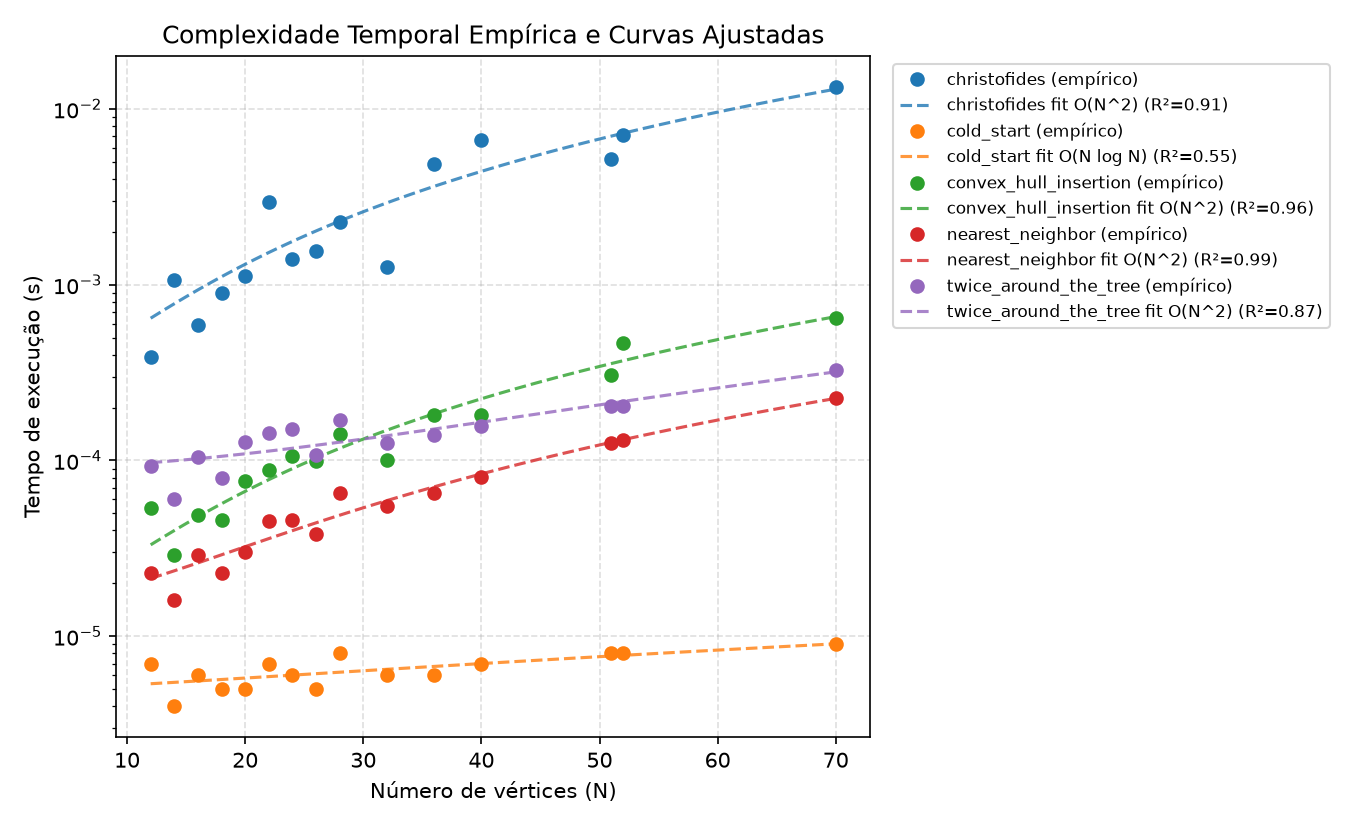
\includegraphics[width=0.92\textwidth]{complexity_time.png}
    \caption{Complexidade temporal empírica e curvas de regressão ajustadas para heurísticas e algoritmos aproximados.}
    \label{fig:complexity_time}
\end{figure}

\begin{figure}[H]
    \centering
    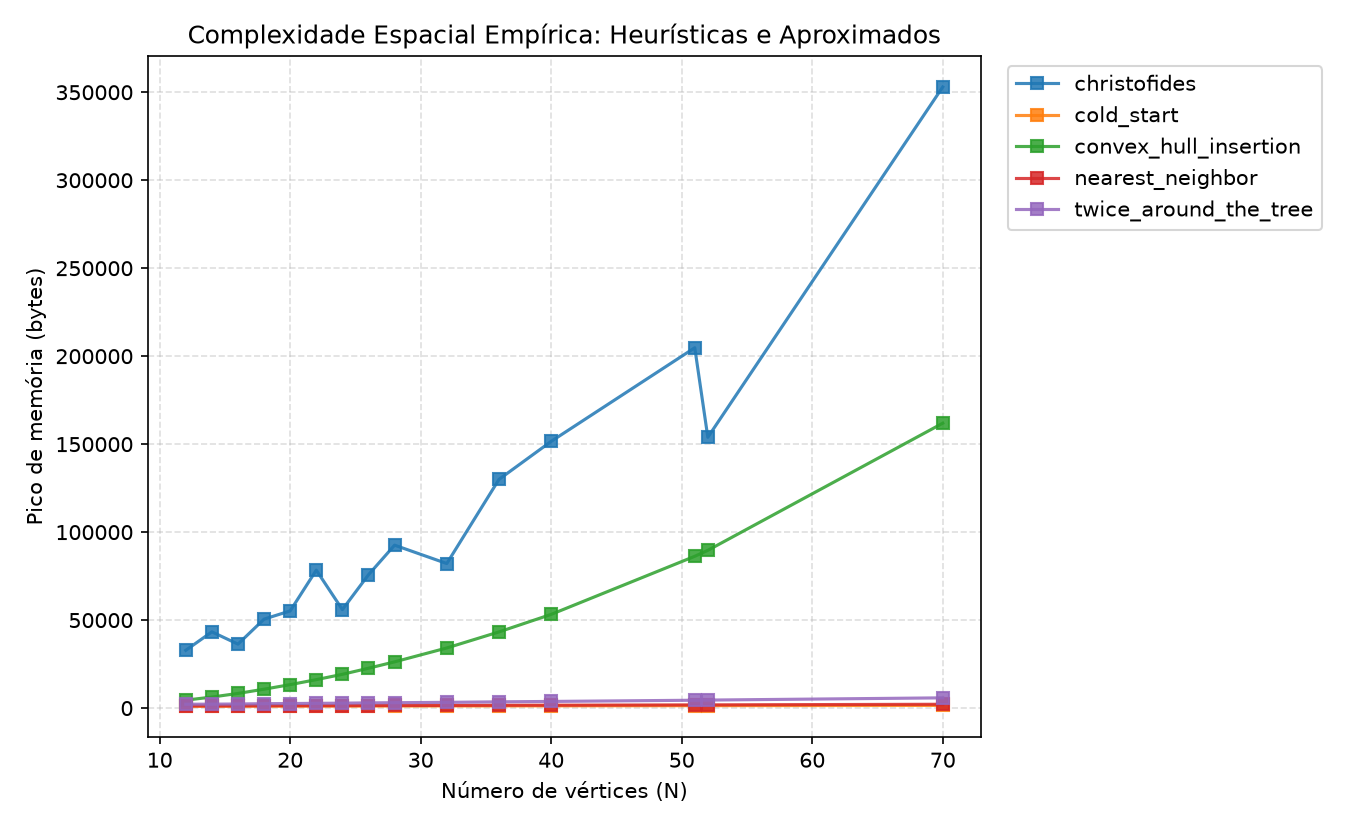
\includegraphics[width=0.92\textwidth]{complexity_memory.png}
    \caption{Pico de memória alocada (\texttt{tracemalloc}) em função de $N$.}
    \label{fig:complexity_memory}
\end{figure}

\begin{figure}[H]
    \centering
    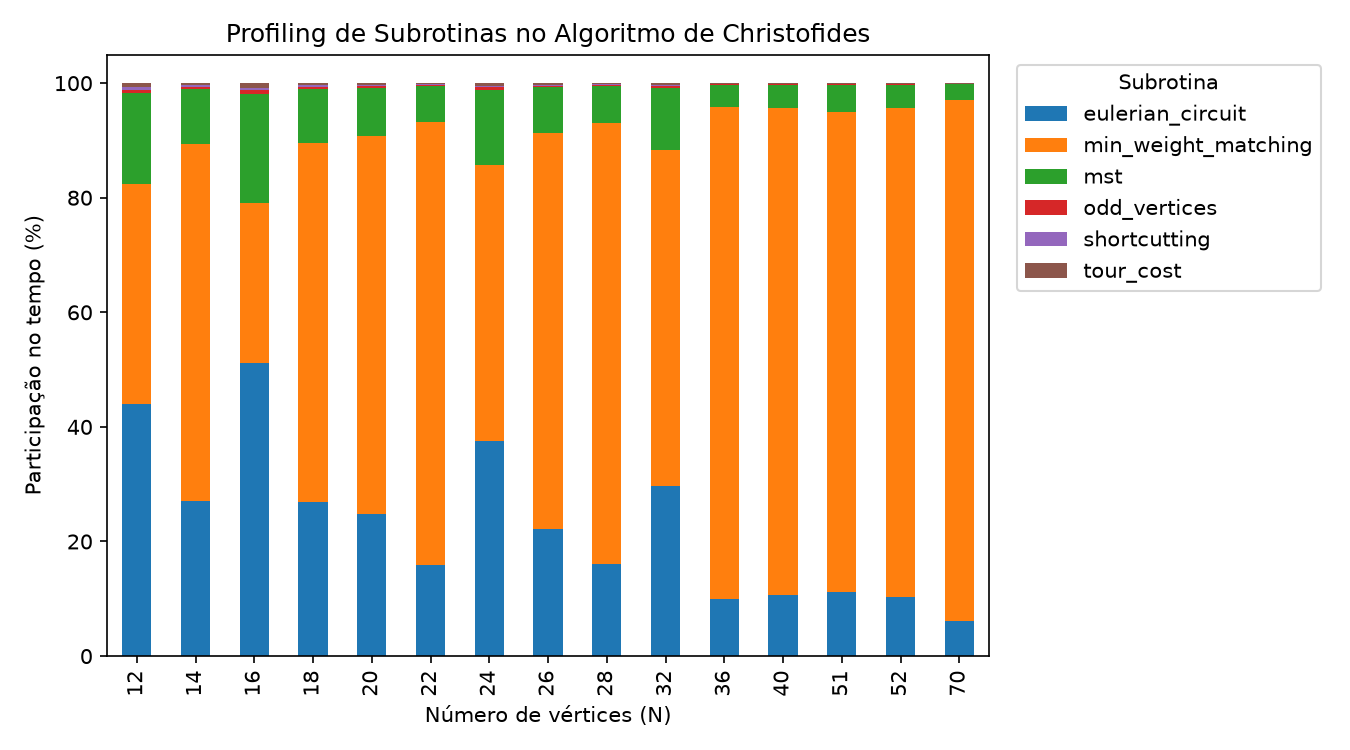
\includegraphics[width=0.92\textwidth]{christofides_subroutines.png}
    \caption{Participação percentual das sub-rotinas no tempo de execução do algoritmo de Christofides.}
    \label{fig:christofides_subroutines}
\end{figure}

\subsection{Impacto do Warm-Start na Eficiência de Poda}
% TODO (Integrante 2): Analisar a Tabela 3 e as Figuras 4 e 5, discutindo o trade-off entre o tempo da heurística inicial e a redução da árvore (ex: convex_hull_insertion reduzindo para 0.699x os nós expandidos em média, chegando a 12x de ganho em eil51_n24).

\begin{table}[H]
\centering
\caption{Desempenho médio das estratégias de \textit{warm-start} nas 9 instâncias resolvidas pelo Branch-and-Bound.}
\label{tab:warm_start}
\resizebox{\textwidth}{!}{%
\begin{tabular}{@{}lcccccc@{}}
\toprule
\textbf{Estratégia} & \textbf{Gap Inicial (\%)} & \textbf{Heur. (ms)} & \textbf{Nós Exp.} & \textbf{Nós Podados} & \textbf{Razão vs. Cold} & \textbf{B\&B (s)} \\ \midrule
1. \texttt{cold\_start}            & 201.41 & 0.006 & 446.624 & 6.773.307 & 1.000 & 77.76 \\
2. \texttt{nearest\_neighbor}      & 18.08  & 0.038 & 446.615 & 6.773.284 & 0.979 & 77.74 \\
3. \texttt{convex\_hull\_insertion}& 2.57   & 0.079 & 430.964 & 6.615.911 & 0.699 & 77.16 \\
4. \texttt{twice\_around\_the\_tree}& 25.16 & 0.115 & 446.338 & 6.771.981 & 0.895 & 76.50 \\
5. \texttt{christofides}           & 9.46   & 1.372 & 446.274 & 6.771.673 & 0.858 & 76.99 \\
\bottomrule
\end{tabular}%
}
\end{table}

\begin{figure}[H]
    \centering
    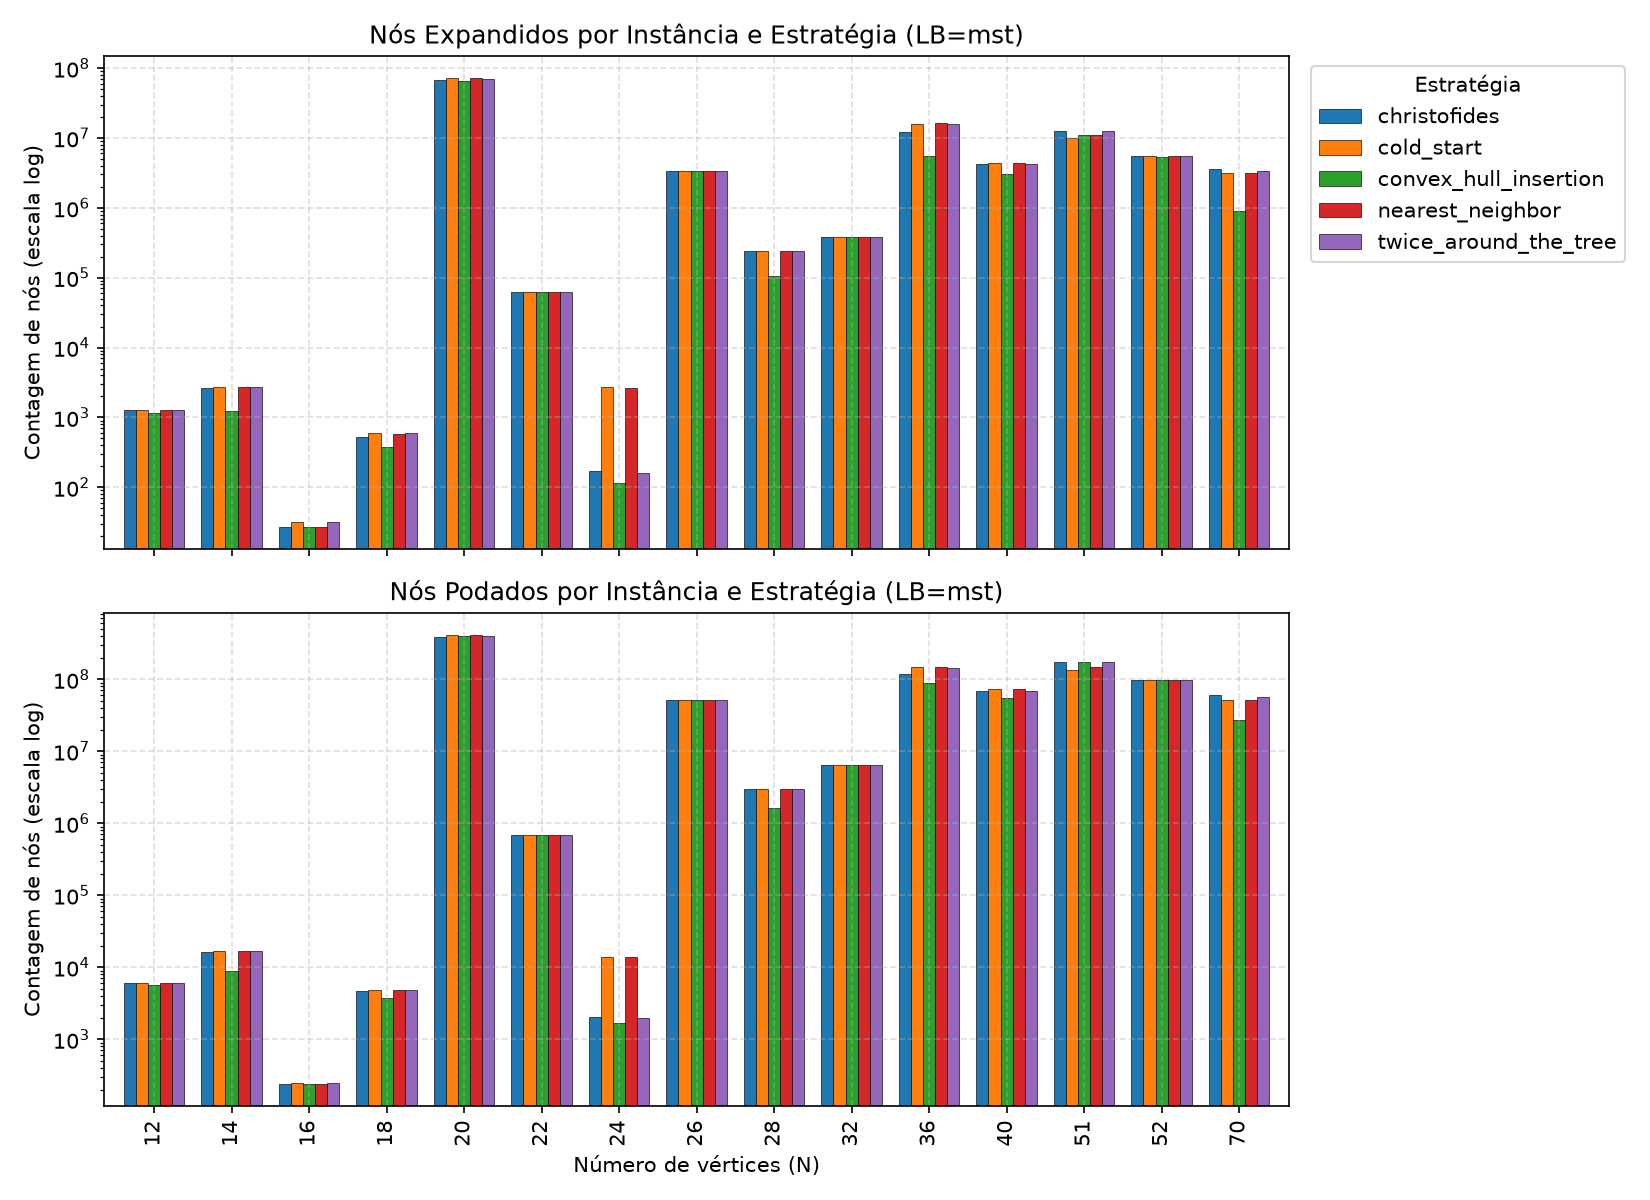
\includegraphics[width=0.95\textwidth]{warmstart_nodes.png}
    \caption{Nós expandidos e nós podados no Branch-and-Bound (\texttt{LB=mst}) por instância e estratégia de inicialização.}
    \label{fig:warmstart_nodes}
\end{figure}

\begin{figure}[H]
    \centering
    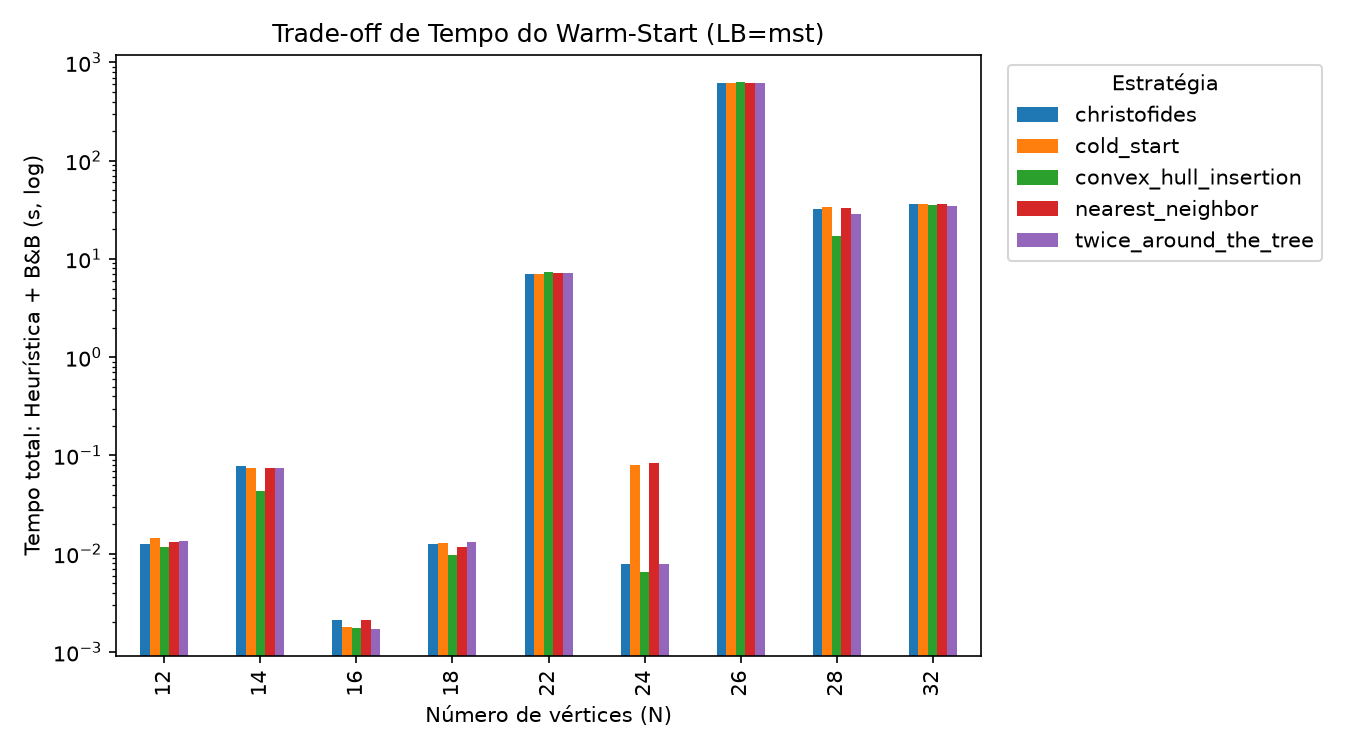
\includegraphics[width=0.92\textwidth]{warmstart_time_tradeoff.png}
    \caption{Tempo total (heurística + Branch-and-Bound) nas 9 instâncias resolvidas dentro do limite de 1800s.}
    \label{fig:warmstart_time_tradeoff}
\end{figure}

\subsection{Análise de Sensibilidade Topológica e Instâncias Adversariais}
% TODO (Integrante 3): Discutir a Figura 6 e as correlações de Spearman:
% - convex_hull_ratio reduz o gap de convex_hull_insertion (rho = -0.708, p = 0.0031) e christofides (rho = -0.624, p = 0.0130);
% - spatial_entropy eleva o gap de nearest_neighbor (rho = +0.646, p = 0.0092) e twice_around_the_tree (rho = +0.621, p = 0.0134);
% - Caso adversarial no B&B: berlin52_n20 (N=20, nn_dist_cv=1.14, timeout 1800s) vs. eil51_n32 (N=32, nn_dist_cv=0.24, 34.6s).

\begin{figure}[H]
    \centering
    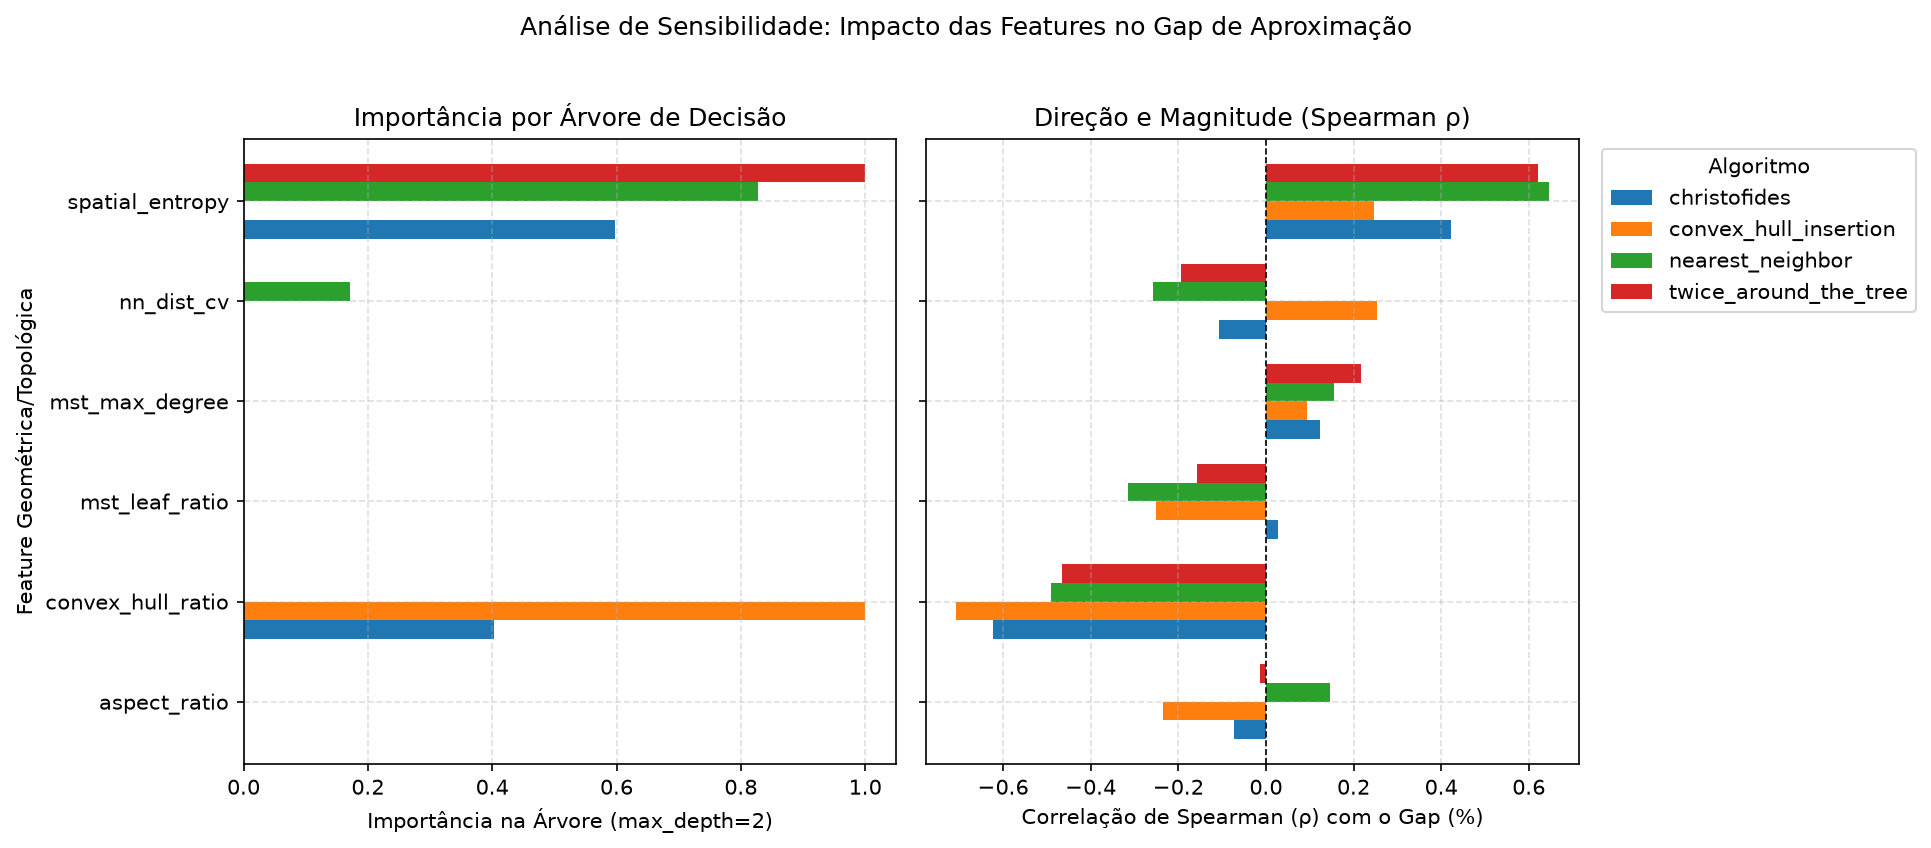
\includegraphics[width=0.95\textwidth]{sensitivity_importance.png}
    \caption{Importância das \textit{features} topológicas na Árvore de Decisão e correlação de Spearman ($\rho$) com o \textit{gap} de aproximação.}
    \label{fig:sensitivity_importance}
\end{figure}

% ==============================================================================
% 5. CONCLUSÕES
% ==============================================================================
\section{Conclusões}
% TODO (Integrante 3): Sintetizar as descobertas empíricas (ponto de colapso do B&B, melhor custo-benefício do convex_hull_insertion no warm-start, gargalo do Matching no Christofides e papel da topologia no gap).

% ==============================================================================
% REFERÊNCIAS BIBLIOGRÁFICAS
% ==============================================================================
\begin{thebibliography}{9}
% TODO: Popular com as referências bibliográficas utilizadas no artigo.
\end{thebibliography}

% ==============================================================================
% APÊNDICE OBRIGATÓRIO (HISTÓRICO DE PROMPTS)
% ==============================================================================
\appendix
\section{Histórico de Prompts Utilizados (Uso de LLMs)}
% TODO (Integrante 3): Registrar ou referenciar o histórico de prompts de LLM consolidado em prompts/.

\end{document}
